% !TEX encoding = UTF-8 Unicode
%!TEX root = memoria.tex
% !TEX spellcheck = es-ES
%%=========================================
\chapter{Metodología}

%%=========================================
\section{Visualización y selección de imágenes}

Como trabajo previo se ha realizado la inspección de las imágenes para escoger aquellas susceptibles a estudio y eliminar aquellas que no cumplen con los criterios para ser incluidas en el estudio.

Para esta tarea se ha hecho uso de las herramientas de visualización de software libre, Mango \footnote{\url{http://rii.uthscsa.edu/mango/}} y MRICron \footnote{\url{http://people.cas.sc.edu/rorden/mricron/index.html}}. La primera de ellas soporta el formato DICOM por lo que ha sido indispensable para un primer acercamiento a los datos.

También se han utilizado estás herramientas para convertir las imágenes y validar algunas de las fases del preprocesado como por ejemplo la extracción del cerebro. Esto es así porque la herramienta es plugable y dispone de algunos plugins, entre los que están la herramienta de extracción de cerebros de FSL \textbf{BET} \footnote{\url{http://rii.uthscsa.edu/mango//plugin_jbet.html}} o el registro lineal automático a una template de referencia con FLIRT \footnote{\url{http://rii.uthscsa.edu/mango//plugin_jflirt.html}}.

Las herramientas de visualización suponen una herramienta fundamental a la hora de validar algunos los procesos involucrados previos al análisis \ref{vis:overlap}.

\begin{figure}[H]
	\centering
	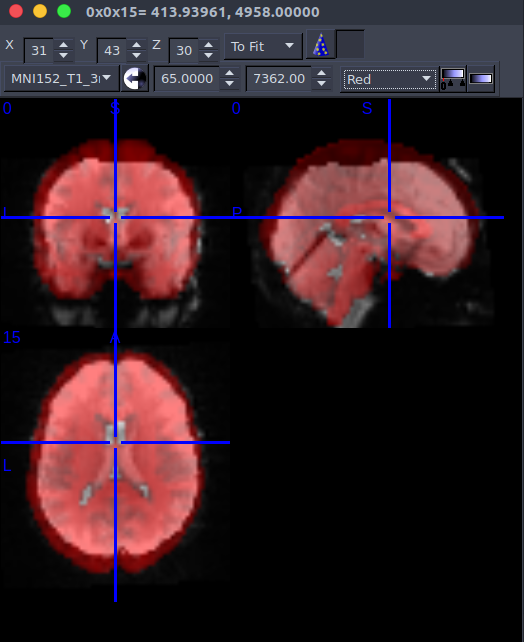
\includegraphics[scale=0.5]{img/overlay.png}
	\caption{Control de registro fMRI}
	\label{vis:overlap}
\end{figure}

Para eliminar el efecto de saturación (los primeros volumenes normalmente tienen una intensidad mayor) se han eliminado los tres primeros volumenes.

\newpage
%%=========================================
\section{Preprocesado}

El pipeline de preprocesado implementado se compone de las siguientes fases

\begin{enumerate}
\item Selección de volumenes para el procesado
\item Extracción del cerebro del volumen anatómico
\item Slice Timming Correction
\item Corrección del movimiento 
%Imagen plots rotación y traslación
\item Co-registro en dos fases
%Imagen overlap del registro a dos fases 
\item Eliminación de artefactos
\item Band pass filter
\item Suavizado Del inglés \textit{smooth}
\end{enumerate}

En la siguiente imagen \ref{preproc:pipeline} se representa gráficamente las distintas fases del preprocesado que han sido implementadas como primera etapa del presente estudio.

\begin{figure}[H]
	\centering
	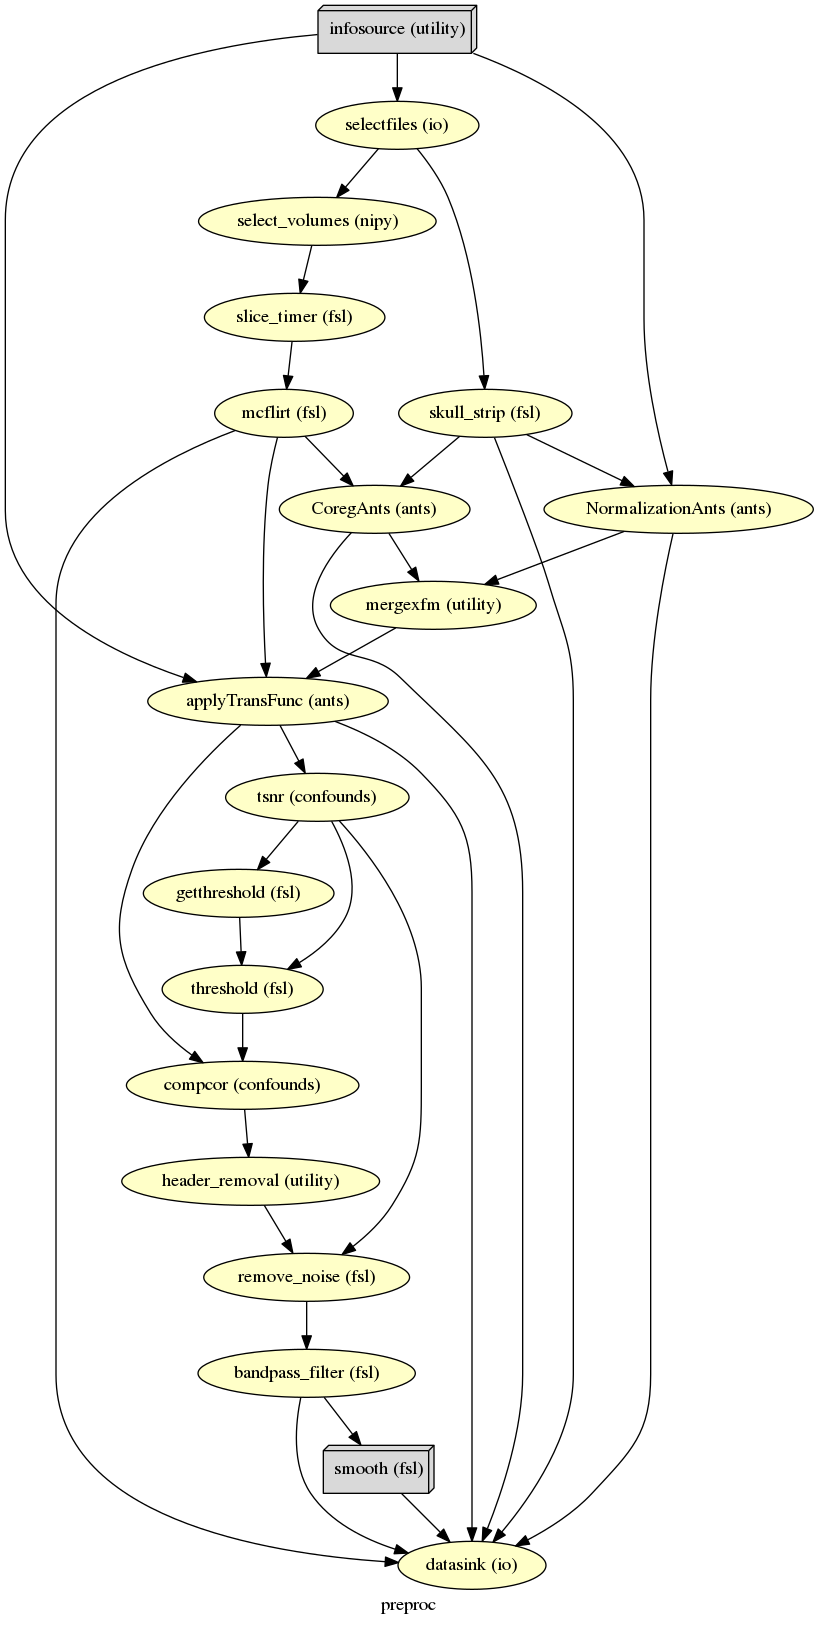
\includegraphics[width=0.5\textwidth]{img/preproc/graph.png}
	\caption{DAG correspondiente con el pipeline de preprocesado}
	\label{preproc:pipeline}
\end{figure}

\subsection{Extracción del cerebro: BET}

 La extracción del cerebro es la primera etapa del preprocesado sobre la imágen estructural. \hyperref[glos:bet]{BET} forma parte de la suite de la herramienta opensource \hyperref[glos:fsl]{FSL} orientada al análisis de imágen cerebral.\\
  Este módulo es el encargado de eliminar los tejidos que no forman parte de la masa cerebral. 
 Se trata de un método automático para la segmentación de imágen de resonancia magnética en tejido cerebral y tejido no cerebral. El método es muy rápido y no requiere de un preprocesamiento previo antes de ser aplicado.\cite{bet}
 En la siguiente \hyperref[preproc:bet] imágen se observa el resultado de aplicar este método a la imágen anatómica de uno de los individuos incluidos en el experimento.
 
 \begin{figure}[H]
	\centering
	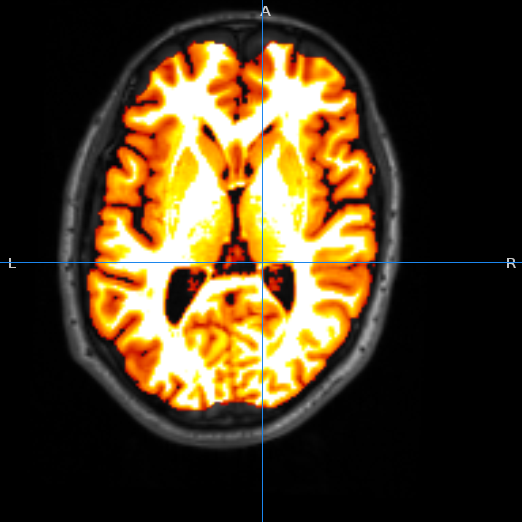
\includegraphics[width=0.5\textwidth]{img/preproc/bet.png}
	\caption{Resultado de aplicar BET en la imagen de uno de los sujetos enfermos del experimento}
	\label{preproc:bet}
\end{figure}

\subsection{Slice Timming Correction}

Con la finalidad de recopilar todos los datos del cerebro, una secuencia típica podría ser adquirir 30 \textit{slices} o más en un intervalo temporal (TR) de tres segundos. Una aproximación trata de utilizar la adquisición en orden ascendente o descentente, la cual obtiene los datos de forma consecutiva. Sin embargo actualmente la mayoría de estudios fMRI usan la adquisición de \textit{slides} por intervalos, en la cual el escaner primero obtiene las imágenes impares, y luego todas las pares.

En el presente estudio se obtienen en orden consecutivo ascentente con un $TR=1.94s$. El método usado por \hyperref[glos:fsl]{FSL} funciona usando la interpolación con ventana de Hanning para cambiar cada serie de tiempo por una fracción apropiada de una TR relativa a la mitad del período TR. Es necesario conocer previamente la metodología de adquisición antes de aplicar el método.

\subsection{Motion correction: MCFLIRT}

 Para la corrección del movimiento se utiliza el módulo MCFLIRT de FSL. Se trata de una herramienta de corrección de movimiento intramodal diseñada para ser aplicada se series temporales obtenidas de las imágenes fMRI. Se trata de una herramienta robusta y precisa, totalmente automatizada. \cite{mcflirt}.
 
\subsection{Normalización en dos fases: ANTs}

\hyperref[glos:ants]{ANTs} es un conjunto de funciones orientadas al estado del arte de registro y segmentación de imagen médica. Su uso más común es para registrar los datos del cerebro en un espacio común estandar, por ejemplo MNI152, como realizamos en el presente estudio. Sin embargo contiene otros métodos para la generación de atlas cerebrales.

Las entradas que se requieren en el registro son:

\begin{itemize}
	\item Imagen fija ode referencia
	\item La imagen a transformar al espacio de la imagen de referencia.
	\item Opcional: Una mascara para reducir el tiempo de computación.
\end{itemize}

En el presente estudio se ha seguido el método de registro en dos fases para normalizar las imágenes fMRI de todos los individuos en el espacio estandar MNI basado en el siguiente algoritmo:



\begin{enumerate}
\item Primero se registra la imágen fMRI en sMRI del mismo sujeto con una transformación lineal
\item Se normaliza la imagen anatómica sMRI en el espacio estandar, utilizando una transformación no lineal basada en el algoritmo \textit{SyN}, un nuevo método de normalización simétrica de imágenes para maximizar la correlación cruzada dentro del espacio de mapas difeomórficos \cite{syn}.
\item Se aplica la transformación generada en el paso uno a las imágenes fMRI obtenidas tras aplicar MCFLIRT. 
\item El último paso aplica la transformación obtenida en la normalización de la imagen anatómica en el espacio estandar a las imágenes obtenidas en el paso anterior. 
\end{enumerate}

Siguiendo este proceso se consiguen resultados confiables \ref{preproc:ants} en la normalización grupal a un espacio estandar.

\begin{figure}[H]
  \begin{subfigure}{\linewidth}
  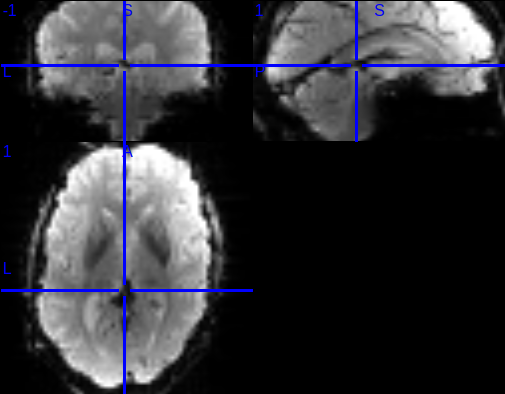
\includegraphics[width=.5\linewidth , height=7cm]{img/preproc/mcf_out.png}\hfill
  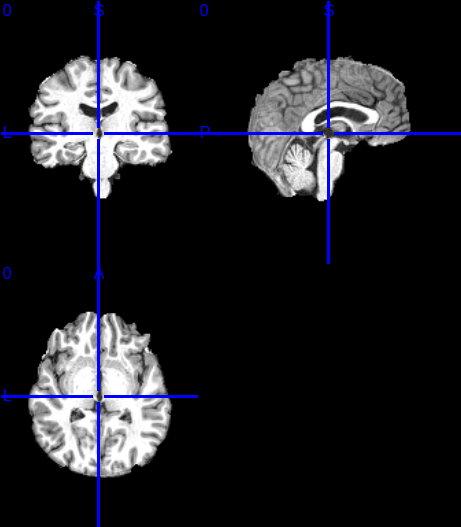
\includegraphics[width=.5\linewidth , height=7cm]{img/preproc/mprage_brain.png}\hfill
  \caption{Imágenes funcional y anatómica previo al registro capturada con MRIcron}
  \end{subfigure}\par\medskip
  \begin{subfigure}{\linewidth}
  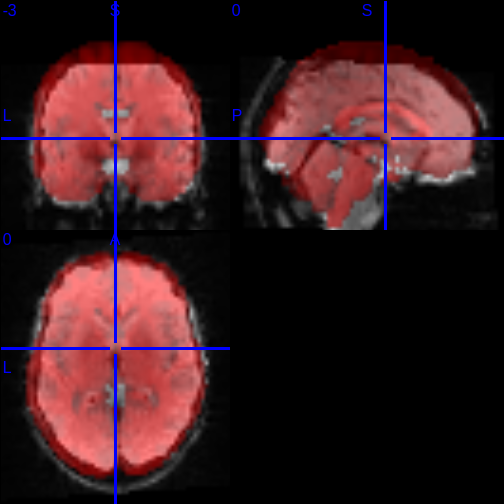
\includegraphics[width=.5\linewidth]{img/preproc/f1.png}\hfill
  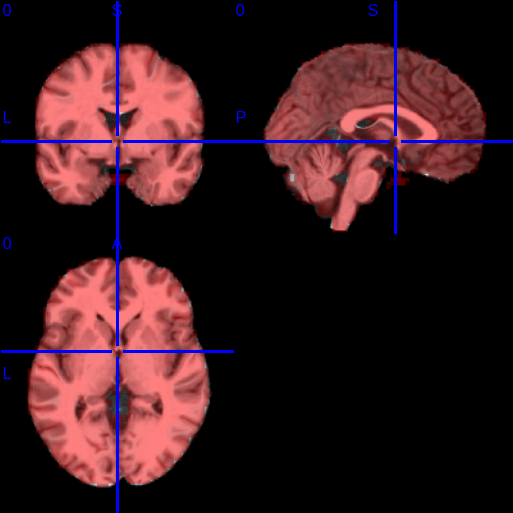
\includegraphics[width=.5\linewidth]{img/preproc/highres2template.png}\hfill
  \caption{Resultados intermedios tras los pasos 1 y 2}
  \end{subfigure}\par\medskip
  \caption{Resultado de aplicar el proceso de normalización en dos fases a un individuo en el experimento. Sobre ambas imágenes se superpone como \textit{overlay} la template}
  \label{preproc:ants}
\end{figure}

\subsection{Eliminación de artefactos: ACompcor}

\subsection{Preprocesado en el dominio de la frecuencia}

%%=========================================
\section{Construcción del mapa funcional}

La construcción del mapa funcional se basa en el análisis \hyperref[glos:ica]{ICA}. Como se ha indicado antes ICA pertenece a los métodos no parámetricos, es un algoritmo de separación de fuente ciega que transforma un conjunto de señales en sus fuentes latentes asociadas. ICA hace no asumen ningún conocimiento a priori de estas fuentes. La única restricción impuesta a a las fuentes es que son estadísticamente independientes y como mucho uno de ellos es gaussiano.\cite{ica}.

En 1998 aparece el primer metodo de generación de mapas de activación basado en ICA \cite{fmriica}. Elresultado de aplicar ICA a un conjunto de datos 4D, como es el caso del fMRI, son las componentes espaciales independientes, cada una de ellas correspondiente con su perfil temporal.


Existen varios algoritmos ICA entre los que nos encontramos el más utilizado \textbf{FastICA}, es un algoritmo de punto fijo que usa la negentropía como función de coste. Tipicamente ICA no se utiliza con el fin de reducir la dimensionalidad si no para separar las señales superpuestas.

%Analizar la influencia del suavizado sobre la generación del mapa funcional con los dos algoritmos, dictlearn & canICA
Retomando lo comentado en el capítulo 2, el suavizado permite identificar los cambios a mayor escala cuanto mayor es el kernel utilizado, ya que éstos se ven más evidentes. En la siguiente secuencia de imágenes se puede apreciar la relación de como afecta en el número de regiones encontradas y el tamaño de estás a medida que aumenta el tamaño del diametro del Kernel utilizado.

\begin{figure}[H]
  \begin{subfigure}{\linewidth}
  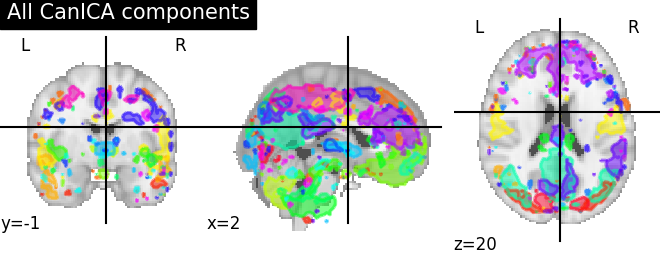
\includegraphics[width=.3\linewidth]{img/canica/canica_None.png}\hfill
  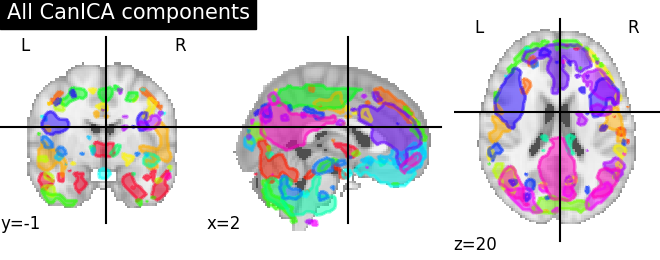
\includegraphics[width=.3\linewidth]{img/canica/canica_4.png}\hfill
  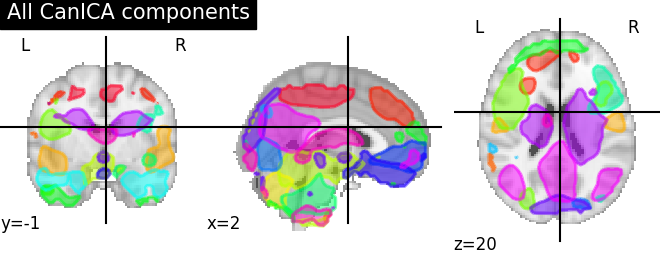
\includegraphics[width=.3\linewidth]{img/canica/canica_8.png}
  \caption{Mapa funcional usando el algoritmo  CanICA con los parámetros de suavizado: None-4mm-8mm}
  \end{subfigure}\par\medskip
  \begin{subfigure}{\linewidth}
  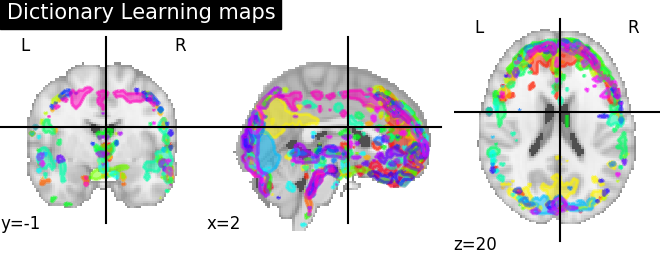
\includegraphics[width=.3\linewidth]{img/canica/dictlearn_None}\hfill
  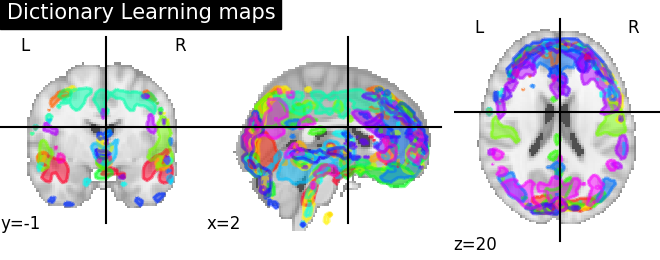
\includegraphics[width=.3\linewidth]{img/canica/dictlearn_4}\hfill
  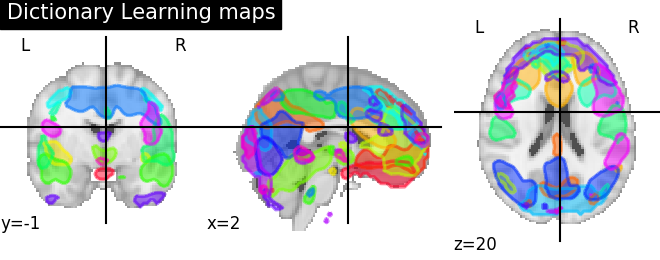
\includegraphics[width=.3\linewidth]{img/canica/dictlearn_8}
  \caption{Mapa funcional usando el algoritmo  DictLearning con los parámetros de suavizado: None-4mm-8mm}
  \end{subfigure}\par\medskip
  \caption{Resultados de diferentes ejecuciones aplicando valores diferentes de suavizado con distintos algoritmos de extracción de mapa funcional}
  \label{preproc:mapa}
\end{figure}

 \textit{Atlas predefinido: } Para el experimento se han tenido en cuenta dos aproximaciones, una a partir de construir el mapa de conectividad inferido a partir de los datos de los individuos enfermos, y otra basada de un atlas MSDL \footnote{\url{https://team.inria.fr/parietal/18-2/spatial_patterns/spatial-patterns-in-resting-state/}} extraido de imágenes fMRI en estado de reposo. Ambas han sido generado utilizando el método \textit{dictionary learning}. Se trata de una variante del algoritmo ICA basado en la asunción de dispersión (\textit{sparsity}) en lugar de la independencia.

\begin{figure}[H]
	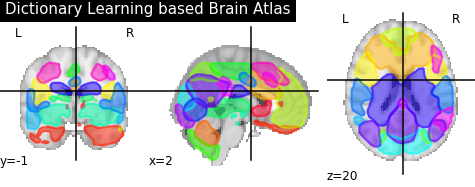
\includegraphics[width=\linewidth, height=\textheight, keepaspectratio]{img/conectividad/dic_prob_atlas_et.png}
	\caption{Atlas inferido de los datos}
	\label{preproc:data_atlas}
\end{figure} 
  
 %%=========================================
\section{Reducción de la dimensionalidad}

En este paso se extraen las series temporales asociadas a cada ROI del atlas de referencia. Esto permite reducir la dimensionalidad agregando los voxels a nivel de ROI. En la imagen \ref{metod:rois} se pueden ver las ROIs obtenidas para con el atlas funcional inferido a partir de los datos de los individuos enfermos.

\begin{figure}[H]
	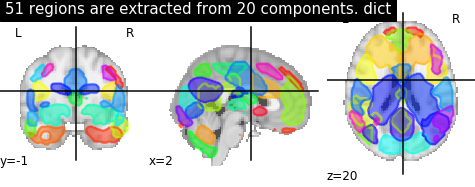
\includegraphics[width=\linewidth, height=\textheight, keepaspectratio]{img/conectividad/dic_rois_et.png}
	\caption{ROIs funcionales obtenidas utilizando Dictionary Learnings en los enfermos de ET}	\label{metod:rois}
\end{figure}

En este paso se extrae las series representativas para cada ROI en cada sujeto para las frecuencias consideradas de interés en la actividad espontánea $0.01-0.08 Hz$ con un filtro de paso banda.\cite{regions}

\begin{figure}[H]
	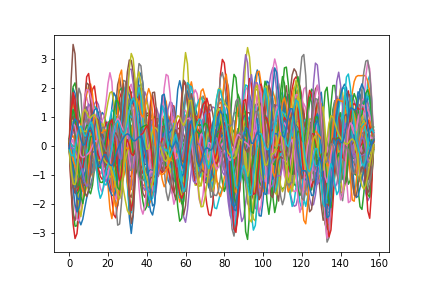
\includegraphics[width=\linewidth, height=\textheight, keepaspectratio]{img/conectividad/ts.png}
	\caption{Series temporales asociadas a cada ROI en un indiviuo}	\label{metod:ts}
\end{figure}

%\begin{figure}[H]
%	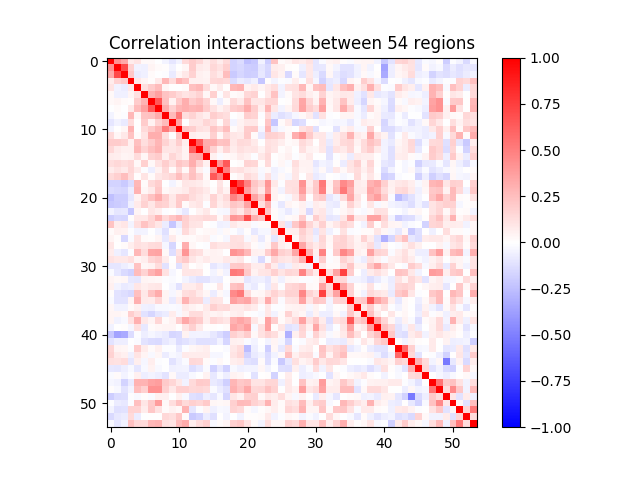
\includegraphics[width=\linewidth, height=\textheight, keepaspectratio]{img/conectividad/matrix.png}
%	\caption{Matriz de conecctividad}
%	\label{preproc:conectividad}
%\end{figure}

%%=========================================
\section{Extracción de parámetros}

%%%=========================================
\subsection{Entropía}

La entropía es un parámetro con múltiples interpretaciones, por ejemplo se suele asociar al desorden o a la escasez de información. Cuando se trata de cuantificar el contenido de información de una distribución de probabilidad, la entropía de Shannon es el parámetro más utilizado.\\

Dada una distribución de probabilidad discreta $P={p_{i}:i=1,\dots,M}$, con $M$ grados de libertad, la entropía de Shannon viene dada por la formula:$$H[P]=-\sum_{i=1}^{M}{p_{i}\ln{p_{i}}}$$

Shannon definió el proceso de entropía como una medida de incertidumbre media de la cantidad de información enviada en un mensae. Cuanto mayor sea el valor de $H[P]$, mayor será la incertidumbre. Por ejemplo si $H[P]= H_{min} =0$, estamos en disposición de predecir con total certeza los resultados de $i$, cuyas probabilidades vienen dadas por $p_{i}$. En este caso el conocimiento del proceso estocástico subyacente descrito por la distribución de probabilidad es máximo. Por el contrario, el conocimiento sobre una distribución uniforme $(P_{e}=\{1/M$, para todo $i=1\dots,M\})$ es mínimo y la incertidumbre máxima cuando 
$$S[P_{e}]=H_{max}=\ln{M}$$ \cite{shannontc}.

Sin embargo este método tiene sus inconvenientes. Por un lado al igual que otros parámetros clásicos descuida las relaciones temporales y por tanto tanto la estructura como los posibles patrones del proceso no se tienen en cuenta. Por otro lado, las medidas de entropía clásica suponen algún conocimiento previo sobre el sistema, se debe proporcionar la distribución de probabilidad asociada al proceso subyacente. La determinación de la distribución de probabilidad más adecuada es un problema fundamental ya que $P$ el el espacio muestral $\omega$ están intimamente ligados. Existen muchos métodos para hayar esta distribución: conteo de frecuencias, procesos basados en la amplitud estadísticas o el análisis de fourier que también será calculado en el presente trabajo. 

Desde el punto de vista del procesado de señal la entropía espectral de Shannon (SSE, Shannon Spectral Entropy)estima en terminos de la uniformidad del espectro de potencia normalizado, la irregularidad de una señal.

Existen estudios basados en la entropía, como el estudio del incremento de la entropía con la edad en la imagen funcional que recoge \cite{Yao2013}. 

\subsubsection{Densidad espectral de potencia}

La distribución de potencia de una señal en terminos de frecuencia, se conoce como densidad espectral de potencia o PSD, puede ser estimada utilizando diferentes variantes de la transformada discreta de fourier (DFT).

Para el cálculo de la \hyperref[glos:psd]{PSD} se utiliza la transformada discreta de Fourier (DFT) para conocer como se encuentra distribuida la potencia en términos de frecuencia. Este análisis constituye un método poderoso que pone en evidencia periodicidades ocultas en una serie temporal. Se trata de una función real positiva de una variable de frecuencia asociada con un proceso estocástico o una función determinística del tiempo que tiene unidades de potencia por hercio (Hz). 

\subsubsection{Entropía espectral de Shannon}

Como hemos mencionado con anterioridad el calculo de la SSE se orienta a estimar la irreguralidad de una señal en terminos de uniformidad del espectro de potencia normalizado.

Una señal muy irregular con mucho ruido asociada a un espectro de potencia plano, con un contenido espectral uniforme obtendría un valor de SSE elevado. Sin embargo un espectro de potencia estrechoformado por unas pocas componentes espectrales tendría una SSE baja. Por tanto consideraremos la SSE como un cuantificador del desorden de la señal, cuyo significado original implica incertidumbre en la información en términos de desorden, discrepancia y diversidad. Además, si comparamos varias señales entre sí, un valor menor de entropía espectral sugiere que esa señal es más regular y predecible

\subsubsection{Entropía de permutación}

La entropía es una poderosa herramienta para el análisis de series temporales, permite describir las distribuciones de probabilidad y la información que contiene un sistema. Sin embargo existe información importante en la dimensión temporal que no suelen analizarse. En los últimos años se ha puesto el foco en la idea de calcular la entropía basada en patrones de permutación, orientada a entender sistemas complejos y caóticos.\cite{pe1}

Al calcular la entropía de permutación tenemos en cuenta la información en el espacio tiempo contenida en la serie temporal. Se trata de un algoritmo robusto, simple para implementar y de bajo coste computacional.

Dada una serie temporal $$ X= \{x_{t}:t=1,\dots,N\}$$ para cada instante $s$ tenemos un registro compuesto por una sequencia de $D$ valores: $$s \rightarrow (x_{s},x_{s+1},\dots,x_{s+D-2}, x_{s+D-1})$$\label{ecuaciones:1}

Donde $n$ es la \textbf{dimensión embebida} o el orden de la permutación y determina cuanta información contiene cada vector. A cada vector se asocia un patrón, definido por la permutación de símbolos $\pi=(r_{0}r{1} \dots r_{n-1})$ de $(01 \dots n-1)$, la cual cumple que:\cite{pe1} $$x_{s+r{0}} \leq x_{s+r_{1}} \dots \leq x_{s+r_{(n-2)}} \leq x_{s+r_{(n-1)}}$$

Dicho de otra forma, los valores de los vectores están ordenados en orden ascendente, y el patrón de permutación $\pi$ se mapea con los valores de los vectores.

La entropía de permutación puede representarse por la ecuación:
$$h_{n}=-\frac{1}{n-1}\sum_{j=1}^{n!}p'_{j}\log{p'_{j}}$$ \label{ecuaciones:3} 

En los últimos años, la entropía de permutación y las métricas relacionadas han surgido como medidas de complejidad apropiadas en el estudio de series temporales de sistemas biológicos, como el cerebro y el corazón.Las razones de este éxito son varias. Por ejemplo, la actividad cerebral espontanea abarca un conjunto de conmutaciones de estado que son continuamente reeditados a través de la corteza, de manera no aleatoria \cite{pe1}.

La ecuación \ref{ecuaciones:1} puede ampliarse con adicionalmente considerando un retardo de inclusión $\tau$ :

$$s \rightarrow (x_{s},x_{s+\tau},\dots,x_{s+\tau(D-2)}, x_{s+\tau(D-1)})$$\label{ecuaciones:2}

Cuando $\tau$ es mayor que uno los valores de las permutaciones no se toman de forma consecutiva, y por tanto se mapean diferentes resoluciones temporales del sistema.

La idea detrás de la entropía de permutación es que los patrones pueden no tener la misma probabilidad de ocurrencia, y por tanto, que esta probabilidad puede revelar información relevante sobre el sistema subyacente \cite{pe1}.

Sin embargo cuando se empieza a utilizar como medida la $PE$ surgen importantes cuestiones como ¿Cuales son los parámetros óptimos?
%%=========================================